% Предишни
% 1 Множества - функции и релации. Декартово произведение на две множества.
% Крайни множества. Изброими и неизброими множества. Ринцип на рекурсивната дефиниция.
% 2 Безкрайни множества и аксиома за избора. Добре наредени множества. Принцип на максимума.
% 3 Топологични пространства. Методи за въвеждане на топологии.Непрекъснати функции и хомеоморфизми.

% ->>>> 4 Операции върху топологични пространства - подпространства, суми, произведения, фактор-пространства.

\section{Подпространство}
\begin{definition}
    Нека $\langle X, \mathcal T_X \rangle$ е топологично пространство и $Y \subseteq X$.
    \begin{equation*}
        \mathcal T_Y = \left\{ U \cap Y \mid U \in \mathcal T_X \right\}
    \end{equation*}
    $\langle Y, \mathcal T_Y\rangle$ е топологично пространство и се нарича подпространство на $\langle X, \mathcal T_X \rangle$ породено от $Y$.
\end{definition}
\begin{lemma}
    Подпространството $\mathcal T_Y$ е топологично пространство.
\end{lemma}
\begin{proof}
    \cite[стр.~89]{munkrestopology}.
\end{proof}
\begin{lemma}
    Нека $\langle X, \mathcal T_X \rangle$ е топологично пространство и $\mathcal B_X$ е база на $\mathcal T_X$.
    \begin{equation*}
        \mathcal B = \left\{ B \cap Y \mid B \in \mathcal B_X \right\}
    \end{equation*}
    $\mathcal B$ е база за подпространството над $Y$.
\end{lemma}
\begin{proof}
    \cite[стр.~89]{munkrestopology}.
\end{proof}
Интересно е кога едно множество е отворено в пространство и съответно в негово подпространство. Възможно е да имаме елемент на подпространството, т.ч. да не е елемент на голямото пространство. \lemref{lem:open-in-subspace} ни показва точно кога едно множество е отворено в двете пространства.
\begin{lemma}\label{lem:open-in-subspace}
    Нека $Y$ е подпространство на $X$, $U$ е отворено в $Y$ и $Y$ е отворено в $X \Rightarrow U$ е отворено в $X$.
\end{lemma}
\begin{proof}
    Лесно се вижда.

    $U$ е отворено в $Y \Rightarrow V \cap Y = U$ за някакво $V$ - отворено в $X$, но $Y$ е отворено в $X$. Значи $U$ е сечение на отворени мн-ва $\Rightarrow U$ е отворено.

    \cite[стр.~89]{munkrestopology}.
\end{proof}
\begin{lemma}
    Нека $Y$ е подпространство на $X$, $U$ е затворено в $Y \iff \exists V $ - затворено в $X:\; U = Y \cap V$.
\end{lemma}
\begin{proof}
    \cite[стр.~94]{munkrestopology}.
\end{proof}
\begin{lemma}
    Нека $Y$ е подпространство на $X$, $U$ е затворено в $Y$ и $Y$ е затворено в $X \Rightarrow U$ е затворено в $X$.
\end{lemma}
\begin{proof}
    \cite[стр.~95]{munkrestopology}.
\end{proof}

\begin{proposition}
    Нека $X$ е топологично пространство, $Y$ - произволно негово подпрстранство, a $Z \subseteq Y$ - произволно подмножество.

    Тогава топологията на подпространство на $Y$ породено от $Z$ и топологията на подпространство на $X$ породено от $Z$ съвпадат.
\end{proposition}

\subsection{Няколко примера}
\begin{example}
    Подпространството на $\R$ породено от $\N$. Това е точно дискретната топология над $\N$.
\end{example}
\begin{proof}
    \begin{equation}
        \mathcal T = \left\{(a; b) \cap \N \mid a, b \in \R\right\}
    \end{equation}
    Това са всички естествени числа между произволни $a$ и $b$.

    Кое да е едноточково множество $\{x\} \subseteq \N$ е елемент на $\mathcal T$, защото $(x-1;x+1) \cap \N = \{x\}$.

    Топологията $\mathcal T$ съдържа всички едноточкови множества, значи е дискретната топология.
\end{proof}
\begin{example}
    Подпространството на $\R$ породено от $\Q$. Не е дискретна топология, понеже $\Q$ е гъсто в $\R$.
\end{example}
\begin{example}
    Подпространството на $\R$ породено от $I = [0; 1]$ - единичният интервал.
\end{example}

\section{Сума на топологии}
За целите на сумата ни трябва фамилия $\mathcal X = \left\{X_i\right\}_{i \in I}$, където $I$ е крайно. Алтернативно $\mathcal X = \left\{X_i\right\}_{i=1}^{n}$. Но тази фамилия не може да е произволна - мн-вата от фамилията трябва да са по двойки непресичащи се.
\begin{equation} \label{eq:disjoint-family}
    i,j \in I:\; X_i \cap X_j = \begin{cases}
        X_i       & , i=j     \\
        \emptyset & , i\neq j
    \end{cases}
\end{equation}
\begin{notation}
    Ще бележим с $\mathcal X$, фамилията:
    \begin{equation*}
        \mathcal X = \left\{X_i\right\}_{i \in I} = \left\{X_i\right\}_{i=1}^{n}
    \end{equation*}
    удовлетворяваща \eqref{eq:disjoint-family}
\end{notation}

Ако имаме топологии $\left\{\mathcal T_i\right\}_{i \in I}$ тогава можем да дефинираме топология над $\mathcal X$
\begin{definition}\label{def:sum-topologies}
    Сума на топологични пространства $\left\{\langle X_i, \mathcal T_i\rangle\right\}_{i \in I}$ ще наричаме топологичното пространство $\langle X, \mathcal T\rangle$, където $X = \bigcup\limits_{i\in I}X_i$ и $\mathcal T = \left\{ U \subseteq X \mid \forall i \in I:\; U \cap X_i \in \mathcal T_i \right\}$
\end{definition}
\begin{fact}
    Отворените множества в сумата $\bigoplus \mathcal X$ са обединенията на отворени множества от отделните топологии.
\end{fact}
\begin{notation}
    Ще бележим сума на топологичните пространства $\mathcal X$ с $\bigoplus \mathcal X$, $\bigoplus\limits_{i\in I} X_i$ или $X_1 \oplus X_2 \oplus \dots \oplus X_n$ (когато топологията е ясна от контекста)
\end{notation}
Разбира се, хубаво е да се изясни, че името "сума на \textbf{топологии}" има смисъл и наистина удовлетворява дефиницията. Наистина "сума на топологии" е топология.

\begin{proposition}
    Ако $X$ може да бъде изразено като фамилия от взаимно непресичащи се отворени подмножества $\mathcal X$, то топологията над $X$ е точно $\bigoplus \mathcal X$
\end{proposition}
\begin{proof}
    \cite[p.~75]{engelking1989general}
\end{proof}
\begin{corollary}
    Значи ако имаме релация на еквивалентност $\sim$ над $X$, то $X/_\sim$ е фамилия от взаимно непресичащи се отворени подмножества, значи
    \begin{equation*}
        X = \bigoplus X/_\sim
    \end{equation*}
    Разбира се, това ще е особена релация на еквивалентност понеже класовете на еквивалентност ще трябва да са отворени множества.
\end{corollary}

\begin{proposition}
    Сумата на топологии е комутативна
\end{proposition}
\begin{proof}
    Достатъчно е да се провери за сума на две пространства. С тривиална индукция се проверява за произволен брой.
\end{proof}

\begin{notation}
    Винаги имаме естественото включване познато от теория на категориите:
    \begin{equation*}
        i_k : X_i \hookrightarrow \bigoplus \mathcal X
    \end{equation*}
\end{notation}
Очевидно е, че $i_k$ е инекция (полезно уточнение)
\begin{proposition}
    $\forall i \in I:\; X_i$ е подпространство на $\bigoplus \mathcal X$
\end{proposition}
\begin{proof}
    Директна проверка на дефинициите
\end{proof}

\subsection{Отслабване на ограничението}
В дефиницията на сума на топологии изискваме всички пространства да са взаимно непресичащи се, но това изглежда не е голямо ограничение понеже за всяка фамилия (не непременно взаимно непресичащи се множества) $\mathcal X$ можем да си построим фамилия от пространства $\mathcal X'$, хомеоморфни на дадените и да зададем $\bigoplus \mathcal X = \bigoplus \mathcal X'$. Например чрез изображението:
\begin{equation}
    \begin{split}
        X \in \mathcal X                    \\
        X \times \{s\} = X' \in \mathcal X' \\
        p_s : X' \to X                      \\
        p_s(x, s) = x                       \\
        p_s = \pi_1
    \end{split}
\end{equation}
Така всяка фамилия от множества има сума (с точност до хомеоморфизъм).
\section{Произведение на топологии}
\begin{definition}
    Нека $\langle X, \mathcal T_X \rangle$ и $\langle Y,\mathcal T_Y \rangle$ са топологични пространства и нека:
    \begin{equation*}
        \mathcal B = \left\{U \times V \mid U \in \mathcal T_X, V \in \mathcal T_Y\right\}
    \end{equation*}
    Тогава $\mathcal B$ е базис на топологично пространство над $X \times Y$.
\end{definition}
Хубаво е да се провери, че наистина е базис.
\begin{proof}
    Проверява се лесно. При съмнение - \cite[p.~86]{munkrestopology}.
\end{proof}
Това е, ако имаме целите топологии, но в повечето случаи предпочитаме да работим с базиси над мн-вата, затова служи следната т-ма:
\begin{theorem}\label{thm:basis-of-times}
    Нека $\mathcal B$ и $\mathcal C$ са базиси на топологии над $X$ и $Y$ съответно. Тогава
    \begin{equation*}
        \mathcal D = \left\{ B \times C \mid B \in \mathcal B, C \in \mathcal C \right\}
    \end{equation*}
    Тогава $\mathcal D$ е базис на топология над $X \times Y$.
\end{theorem}
\begin{proof}
    \cite[p.~87]{munkrestopology}.
\end{proof}
\begin{example}
    Стандартната топология $\R^2$ е стандартната топология на $\R$ $\times$ стандартната топология на $\R$. Но това е голямо множество. \thref{thm:basis-of-times} ни казва, че можем да работим с базиса от всички отворени правоъгълници (а това е доста по-малко мн-во).
\end{example}
\begin{example}
    Още една известна топология е $\R_l \times \R_l$ с името "равнина на Соргенфрей".
\end{example}
\begin{notation} 
    Нека $A_i, i \in I$ са мн-ва за някакво индексно мн-во $I$.
    
    $\pi_k : \prod\limits_i A_i \to A_k$ е стандартната проекция на $k$-тия елемент от Декартовото произведение.
\end{notation}
Тривиално наблюдение е, че $\forall k \in I: \pi_k$ е сюрективна. Тогава можем да конструираме:
\begin{equation*}
    \pi_k^{-1}(U) = A_1 \times \dots \times A_{k-1} \times U \times A_{k+1} \times \dots \times A_k \text{ за } U \subseteq A_k
\end{equation*}
От тук произтича и следната теорема:
\begin{theorem}
    \begin{equation*}
        \mathcal B = \left\{ \pi_1^{-1}(U) \mid U \in \mathcal T_X \right\} \cup \left\{ \pi_2^{-1}(V) \mid V \in \mathcal T_Y \right\}
    \end{equation*}
    $\mathcal B$ е подбазис на топологията на $X \times Y$.
\end{theorem}
\begin{proof}
    Лесно се забелязва, че:
    \begin{equation*}
        \forall U \in \mathcal T_X, V\in \mathcal T_Y : \pi_1(U) \cap \pi_2(V) = U \times V
    \end{equation*}
    което е отворено в $X \times Y$.
    
    \cite[p.~88]{munkrestopology}.
\end{proof}

\subsection{Обобщение}
Дефинирахме операцията за 2 пространства, но нищо не ни спира да го обобщим за произволен брой:
\begin{definition}
    Нека $\mathcal X = \left\{X_i\right\}_{i \in I}$ е фамилия от топологични пространства.

    Дефинираме $\prod \mathcal X = \prod\limits_{i \in I}X_i$ да бъде топологията, която е произведение на пространствата от фамилията.
\end{definition}
\begin{proposition}
    Произведението на топологии е асоциативно.
\end{proposition}
\begin{proof}
    Тривиално се проверява използвайки асоциативността на Декартовото произведение.
\end{proof}
\begin{notation}
    Ако $\forall i \in I,\ X_i = X$ за някакво фиксирано $X$ и $|I| = n$, тогава $\prod \mathcal X $ бележим с $X^n$ и се нарича \textbf{$n$-та степен на $X$}. Ако $|I| = \aleph_0$, то $\prod \mathcal X $ бележим с $X^\omega$ (не успях да намеря превод на \emph{$\omega$-tuple}).
\end{notation}
Естествено наблюдение е, че всички доказани твърдения са верни за произволни произведения на пространства.

\subsubsection{Генериране на обобщеното произведение}
Интересно е как могат да се генерират произведенията. За това ни помага следното твърдение:
\begin{proposition}
    Нека $\mathcal X = \left\{X_i\right\}_{i\in I}$ е фамилия от пространства, а $\mathcal W = \left\{W_i\right\}_{i\in I}$, т.ч. $\forall i\in I:\; W_i$ е отворено в $X_i$ и само за краен брой $W \in \mathcal W,\; W \subseteq X \in \mathcal X$ е вярно, че $W \neq X$.

    Тогава $\mathcal W$ е базис за $\prod \mathcal X$.
\end{proposition}
\begin{proof}
    \cite[p.~77]{engelking1989general}.
\end{proof}
\section{Фактор-пространство}
Факторизирането е познато от други области като линейната алгебра и теория на групите, където разглеждаме множество елементи като един под действието на някакво изображение. По подобен начин ще разглеждаме и фактор-пространствата в топологията.

В геометричната интерпретация на топологията, факторизацията има смисъл на деформация и "залепване" на краищата.

\begin{example}
    Ако разгледаме квадрат и факторизираме като разглеждаме следните обекти като еквивалентни (ще покажем защо използваме точно тази дума по-долу в текста):

    \begin{itemize}
        \item Четирите ъгъла на квадрата
        \item Две по две успоредните страни
        \item Вътрешността на квадрата
    \end{itemize}

    Така полученото факторизиране всъщност е хомеоморфно на тор.
    \begin{figure}[H]
        \centering
        \includegraphics[width=\textwidth]{resources/torus.png}
        \caption{Визуално представяне на факторизацията (взето от \cite[стр.~140]{munkrestopology})}
    \end{figure}
\end{example}

\subsection{Факторно изображение}
\begin{definition}
    Нека $X, Y$ са топологични пространства.
    
    $p: X \to Y$. $p$ е факторно изображение $\bydef$ p е сюрекция и $\forall U \in Y$ - отворено множество: $p^{-1}(U)$ е отворено множество в $X$.
\end{definition}
\begin{notation}
    В тази секция употребяваме факторно (изборажение) като превод на "quotient map" или "strong continuity".
\end{notation}
\begin{definition}
    Нека $X$ е топологично пространство.
    
    $C \subseteq X$ е наситено(спрямо сюрективно изображение $p: X\to Y$) $\bydef$ $\forall y \in Y:\; p^{-1}(\{y\}) \cap C \neq \emptyset \rightarrow p^{-1}(\{y\}) \subseteq C$  .
\end{definition}
\begin{notation}
    Когато е ясно от контекста ще пропускаме "спрямо сюрективно изображение \dots".
\end{notation}
Иначе казано, $C$ е наситено точно тогава когато има такова подмножество на $U \subseteq Y$, че $p^{-1}(U) = C$.

Значи можем еквивалентно да дефинираме факторно изображение чрез наситени множества по следния начин:
\begin{proposition}
    $p: X \to Y$ е факторно изображение $\iff$ $p$ е непрекъснато изображение и изобразява наситените отворени множества на $X$ в отворени множества на $Y$.
\end{proposition}

Лесно може да се съобрази, че:
\begin{proposition}
    Нека $X, Y$ са топологични пространства.

    $p: X \to Y$ е сюрективно непрекъснато отворено/затворено изображение $\Rightarrow$ $p$ е факторно изображение.
\end{proposition}
\begin{remark}
    Това е достатъчно, но не е необходимо условие, т.е. има факторни изображения, които не са нито отворени, нито затворени.
\end{remark}
\begin{proof}
    Нека разглеждаме $\pi_1: \R \to \R$. Нека $A$ е подпространство на $\R \times \R$, т.ч.:
    \begin{equation}
        A = \{\langle x, y \rangle \mid x \geq 0 \lor y=0\}
    \end{equation}
    Нека $q : A \to \R$ дефинирано като рестрикцията на $\pi_1$ върху $A$.

    Тогава твърдим, че $q$ не е нито отворено, нито затворено изображение.

    \begin{itemize}
        \item[(не е отворено)] Търсим такова отворено множество $X \subseteq A$, че $q(X)$ не е отворено в стандартната топология на $\R$.
        
        Нека $X = [0; 1) \times \{0\}$. Тогава:
        \begin{equation}
            q(X) = [0; 1)
        \end{equation}
        Но това не е отворено множество $\R$.

        \item[(не е затворено)] Търсим такова затворено множество $X \subseteq A$, че $q(X)$ не е затворено в стандартната топология на $\R$.
        
        Нека $X = [0; 1) \times \{0\}$. Тогава:
        \begin{equation}
            q(X) = [0; 1)
        \end{equation}
        Но това не е затворено множество $\R$.
    \end{itemize}
    Значи можем да използваме един и същи контрапример за двата случая понеже интервалът $[0; 1)$ не е нито отворен, нито затворен.

    Не можем да изразим като крайно/безкрайно обединение и сечение на отворени интервали - няма как да "затворим" отляво интервала.
    \begin{equation}
        [0; 1) = \{0\} \cup (0; 1)
    \end{equation}
    Защото $\{0\}$ не е отворено множество.

    Допълнението му също не е отворено множество:
    \begin{equation}
        \overline{[0; 1)} = (-\infty; 0) \cup [1; \infty) = \bigcup_{n \in \N} (-n;0) \cup \{1\} \cup \bigcup_{n\in\N} (1+n;\infty)
    \end{equation}
    Защото $\{1\}$ не е отворено множество.
\end{proof}

\subsection{Фактор-топология дефинирана от изображение}
\begin{definition}
    Нека $X$ е топологично пространство, $A$ е произволно множество, $p: X \to A$ e сюрективно изображение.

    Тогава най-малката топология $\mathcal T$ над $A$, т.ч. $p$ е факторно изображение, се нарича Фактор-топология породенa от $p$.

    \begin{equation}
        \mathcal T = \{U \subseteq A \mid p^{-1}(U) \in \mathcal T_X\}
    \end{equation}
\end{definition}
Лесно се проверява, че е топология - при съмнение \cite[стр.~138]{munkrestopology}.

\begin{example}
    Нека $x \in \R$ е произволно и $A = \{a, b, c\}$ и $p: \R \to A$ дефинирано по следния начин:
    \begin{equation}
        p(y) = \begin{cases}
            a &, y > x\\
            b &, y < x\\
            c &, y = x
        \end{cases}
    \end{equation}

    Визуално топологията изглежда по следния начин:
    \begin{figure}[H]
        \centering
        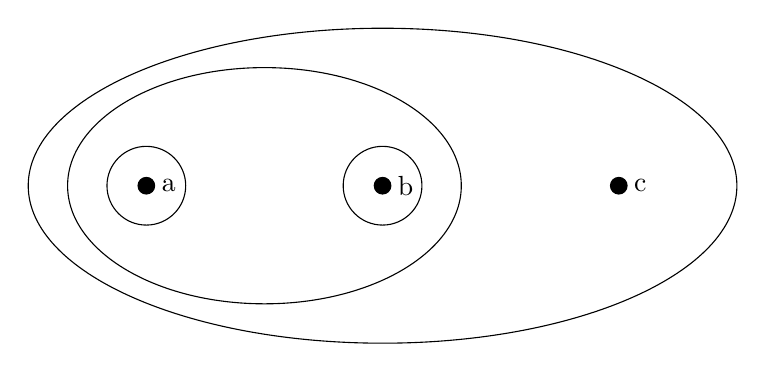
\begin{tikzpicture}
            \filldraw (-3, 0) circle (3pt) node [xshift = 2pt, anchor=west]{a};
            \filldraw (0, 0) circle (3pt) node [xshift = 2pt, anchor=west]{b};
            \filldraw (3, 0) circle (3pt) node [xshift = 2pt, anchor=west]{c};

            \draw (-3, 0) circle (0.5);
            \draw (0, 0) circle (0.5);
            % \draw (3, 0) circle (0.5);
            \draw (-1.5, 0) ellipse (2.5 and 1.5);
            \draw (0, 0) ellipse (4.5 and 2);
        \end{tikzpicture}
        \caption{Визуално представяне на топологията породена от $p$}
    \end{figure}
    
    \begin{remark}
        Забелязваме, че $c$ е елемент единствено на цялото множество - това се дължи на факта, че не можем да произведем полузатворен интервал с край $x$ - от вида $(v; x]$ или $[x; u)$.
    \end{remark}
    
    \begin{remark}
        Също полученото фактор-пространство не е Хаудосрфово.

        $a$ и $c$ не могат да бъдат отделени една от друга, защото $a$ е елемент на $\set{a}, \set{a, b}, A$, доката $c$ е елемент само на $A$. Няма околности, които да са непресичащи се.
    \end{remark}
\end{example}

\subsubsection{Композиция}
Лесно се проверява, че композицията запазва силната непрекъснатост благодарение на следния факт:
\begin{equation}
    p^{-1}(q^{-1}(x)) = (q \circ p)^{-1}(x)
\end{equation}
\begin{proposition}
    Нека $X_1, X_2, X_3$ са топологични пространства, $p_i: X_i \to X_{i+1}$ е факторно изображение за $i \in \{1, 2\}$.

    Тогава $p_1 \circ p_2 : X_1 \to X_3$ е факторно изображение.
\end{proposition}

\subsubsection{Произведение}
Декартовото произведение не винаги запазва силната непрекъснатост.
\begin{proof}
    Конструкция е.
    \cite[стр.~143]{munkrestopology}
\end{proof}

\subsection{Фактор-пространство дефинирано от релация на еквивалентност}
\subsubsection{Припомняне от теория на множествата}
\begin{definition}
    Нека $X$ е множество, а $\sim$ релация над $X$.

    $\sim$ е релация на еквивалентност $\bydef$ $\sim$ е рефлексивна, симетрична и транзитивна.
\end{definition}
\begin{definition}
    Нека $X$ е множество, а $\sim$ релация на еквивалентност над $X$. Клас на еквивалентност породен от $x \in X$ наричаме множество от всички елементи еквивалентни на $x$:
    \begin{eqnarray}
        [x] \overset{def}{=} \{y \in X \mid x \sim y \}
    \end{eqnarray}
\end{definition}

\begin{definition}
    Нека $X$ е множество, а $\sim$ релация на еквивалентност над $X$. $X$ факторизирано по $\sim$ наричаме фамилия от множества съставена от всички класове на еквивалентност:
    \begin{eqnarray}
        X/_\sim = \left\{[x] \mid x \in X\right\}
    \end{eqnarray}
\end{definition}

\begin{fact}
    Лесно се проверява, че два класа или съвпадат, или са непресичащи се:
    \begin{eqnarray}
        [x] \cap [y] = \begin{cases}
            [x] = [y] &, x \sim y\\
            \emptyset &, x \not\sim y
        \end{cases}
    \end{eqnarray}
\end{fact}

\begin{corollary}
    $X/_\sim$ е разбиване на $X$.
\end{corollary}
\begin{corollary}
    $X/_\sim$ поражда естествено сюрективно изображение $p: X \to X/_\sim,\; x \mapsto [x]$.
\end{corollary}

\subsubsection{Фактор-пространство}
\begin{definition}
    Нека $X$ е множество, $\sim$ е релация на еквивалентност над $X$, с естествено влагане $p: X \to X/_\sim$. С топологията породена от $p$, $X/_\sim$ се нарича фактор-пространство.
\end{definition}
\begin{proposition}
    Двете дефиниции за фактор-пространство са еквивалентни.
\end{proposition}
\begin{fact}
    Относно естественото включване, изображенията в двете посоки изглеждат по следния начин:

    От множеството към фактор-множеството:
    \begin{equation}
        p(X) = p(\{x_1, x_2, \dots, x_n, \dots\}) = \{[x_1], [x_2], \dots, [x_n], \dots\} = U
    \end{equation}

    От фактор-множеството към множеството:
    \begin{equation}
        p(U) = p(\{[x_1], [x_2], \dots, [x_n], \dots\}) = \bigcup_{[x] \in U} [x]
    \end{equation}
\end{fact}

\subsubsection{Относно подпространства}
\begin{theorem}
    Нека $X, Y$ са топологични пространства, $p: X \to Y$ е факторно изображение, $A \subseteq X$ е наситено подмножество. 

    Нека $q = p\mid_A, q: A \to p(A)$.
    \begin{itemize}
        \item Ако $A$ е отворено/затворено $\Rightarrow$ $q$ е факторно
        \item Ако $p$ е отворено/затворено изображение $\Rightarrow$ $q$ е факторно
    \end{itemize}
\end{theorem}
\begin{proof}
    \cite[стр.~140]{munkrestopology}.
\end{proof}

\subsection{Непрекъснати функции над фактор-пространство}

Подобно на \thref{th:sum-continuous} ще се интересуваме от това кога една функция е непрекъсната по отношение на това къде е дефинирана или нейните стойности.

Съответната на \thref{th:sum-continuous} по отношение на фактор-пространства е следната:
\begin{theorem}\label{th:factor-continuous}
    Нека $X, Y, Z$ са топологични пространства, $p: X \to Y$ е факторно изображение и $g: X \to Z$ е изображение, т.ч.
    \begin{equation}
        \exists z \in Z,\ \forall y \in Y:\; g(p^{-1}(\{y\})) = z
    \end{equation}
    т.е. $g$ е константа над всички множества от вида $p^{-1}(\{y\})$.

    Тогава $g$ поражда функция $f: Y \to Z,\ f \circ p = g$.
    \begin{itemize}
        \item $f$ е непрекъсната $\iff$ $g$ е непрекъсната
        \item $f$ е факторно $\iff$ $g$ е факторно
    \end{itemize}

    \begin{figure}[H]
        \centering
        \begin{tikzpicture}[
        node distance=3cm,
        auto
        ] 
           \node[state] (X) {$X$}; 
           \node[state] (Y) [below of = X] {$Y$}; 
           \node[state] (Z) [right of = Y]  {$Z$};
            \path[->] 
            (X) edge  node {$p$} (Y)
                edge  node {$g$} (Z)
            ;
            \path[->, dashed]
            (Y) edge node {$f$} (Z)
            ;
        \end{tikzpicture}
        \caption{Диаграмата е комутативна по формулировката на теоремата}
    \end{figure}
\end{theorem}
\begin{proof}
    \cite[стр.~142]{munkrestopology}.
\end{proof}
\begin{corollary}
    Нека $g: X \to Z$ е сюрективно непрекъснато изображение и $X^*$ е такова, че:
    \begin{equation}
        X^* = \{g^{-1}(\{z\}) \mid z \in Z\}
    \end{equation}
    $X^*$ е фактор-пространство породено от подходяща функция $p$.

    Тогава по \thref{th:factor-continuous} знаем, че има породена биективна\footnotemark  функция $f: X^* \to Z$, която е хомеоморфизъм, т.с.т.к. $g$ е факторно.  
    \footnotetext{праобразът (като множество) на дадено $z \in Z$ е напълно достатъчно, за да се опрелени еднозначно}.
\end{corollary}
\begin{proof}
    \cite[стр.~142-143]{munkrestopology}.
\end{proof}

\subsection{Примери}
Допълнителни примери за факторни изображения и фактор-пространства по релация на еквивалентност. Вж. \cite[стр.~144-145]{munkrestopology}.
\begin{example}
    Нека $X$ е топологично пространство и $A \subset X$, тогава $id_X\mid_A$ е факторно изображение.
\end{example}
\begin{example}
    Дефинираме релация $\sim$ над $\R^2$:
    \begin{equation}
        \langle x_0, y_0 \rangle \sim \langle x_1, y_1 \rangle \bydef x_0 + y_0^2 = x_1 + y_1 ^2
    \end{equation}
    Очевидно е релация на еквивалентност основавайки се на факта, че $=$ е релация на еквивалентност.

    Да разгледаме няколко класа на еквивалентност:
    \begin{equation}
        [\langle 0, 0 \rangle] = \{ \langle -x^2, x \rangle \mid x \in \R_0^+\}
    \end{equation}
    Това е графиката на $x^2$ завъртяна с $\frac{\pi}{2}$.
    \begin{equation}
        [\langle 0, 1 \rangle] = \{ \langle -x^2 + 1, x \rangle \mid x \in \R_0^+\}
    \end{equation}
    Това е графиката на $x^2 - 1$ завъртяна с $\frac{\pi}{2}$.

    Забелязваме, че:
    \begin{equation}
        a\in \R:\; [\langle 0, a \rangle] = \{ \langle -x^2 + a^2, x \rangle \mid x \in \R_0^+\}
    \end{equation}

    Да се опитаме да варираме първата координата:
    \begin{equation}
        [\langle 1, 0 \rangle] = \{ \langle -x^2 + 1, x \rangle \mid x \in \R_0^+\}
    \end{equation}
    \begin{equation}
        [\langle 2, 0 \rangle] = \{ \langle -x^2 + 2, x \rangle \mid x \in \R_0^+\}
    \end{equation}
    \begin{equation}
        a\in \R:\; [\langle a, 0 \rangle] = \{ \langle -x^2 + a, x \rangle \mid x \in \R_0^+\}
    \end{equation}
    \begin{equation}
        [\langle 1, 1 \rangle] = \{ \langle -x^2 + 2, x \rangle \mid x \in \R_0^+\}
    \end{equation}
    \begin{equation}
        [\langle 2, 1 \rangle] = \{ \langle -x^2 + 3, x \rangle \mid x \in \R_0^+\}
    \end{equation}
    \begin{equation}
        a \in \R:\; [\langle a, 1 \rangle] = \{ \langle -x^2 + a + 1, x \rangle \mid x \in \R_0^+\}
    \end{equation}
    \begin{equation}
        a \in \R:\; [\langle a, 2 \rangle] = \{ \langle -x^2 + a + 4, x \rangle \mid x \in \R_0^+\}
    \end{equation}
    Забелязваме вече шаблона, затова твърдим:
    \begin{equation}
        a, b \in \R:\; [\langle a, b \rangle] = \{ \langle -x^2 + a + b^2, x \rangle \mid x \in \R_0^+\}
    \end{equation}
\end{example}
\subsection{Топология породена от наредба и подпространство}
Нека имаме топология породена от наредба над $\langle X, < \rangle$ и едно подмножество $Y \subseteq X$. Множеството $Y$ е наредено от $< \mid_Y$. Значи има топология породена от наредба за $\langle Y, < \rangle$, но може да се случи така, че да не съвпада с топологията на $Y$ като подпространство на $X$.
\begin{example}
    Нека $X = \R, Y = [0; 1) \cup {2}$. Отбелязваме, че $Y \subseteq \R$.
    
    Топологията на $Y$ като подпространство $\mathcal T_{sub}$ съдържа $\{2\}$, защото може да се представи като сечение на отворено множество от стандартната топология на $\R$ с $Y$:
    \begin{equation}
        \{2\} = Y \cap \left(\frac{3}{2}; \frac{5}{2}\right)
    \end{equation}

    Обаче ако разгледаме топологията на $Y$ породена от стандартната наредба на $\R$ - $\mathcal T_<$ с базис $\mathcal B_<$-  ще открием, че $\{2\}$ не е отворено множество. Всеки елемент на $\mathcal B_<$, който съдържа 2 по необходимост ще съдържа и други числа. Нека $2 \in S, S \in \mathcal B_<$:
    \begin{equation}
        S = (a; 2] \Rightarrow 2 \neq \frac{a + 2}{2} \in S
    \end{equation}
    Значи няма как да е отворено множество в $\mathcal T_<$, защото всяко отворено множество ще съдържа числа по-малки от 2.
\end{example}

\subsubsection*{Има случаи, обаче, когато двете съвпадат:}
\begin{example}
    Нека $X = \R,\ Y = [0; 1] = I$. Известно ни е, че $I \subset \R$.

    Като подпространство $\langle I, \mathcal T_{sub}\rangle$ има базис:
    \begin{equation}
        \mathcal B_{sub} = \left\{(a; b) \cap I\mid a < b\right\}
    \end{equation}
    Знаем, че за $(a; b) \cap I$ имаме няколко случая:
    \begin{equation}
        (a; b) \cap I = \begin{cases}
            (a; b)      & a, b \in I \\
            [0; b)      & a \notin I, b \in I\; (\star)\\
            (a; 1]      & a \in I, b \notin I\; (\star)\\
            I           & a < 0, b > 1 \\
            \emptyset   & a, b < 0 \lor a, b > 1 \\
        \end{cases}
    \end{equation}

    По дефиниция всичките са отворени в $\langle I, \mathcal T_{sub} \rangle$, означените със $(\star)$ не са отворени в $\R$. 
    
    Но това формира базиса на топологията като подпространство, което съвпада с базиса на топологията породена от наредбата $<$ над $I$:
    \begin{equation}
         \mathcal B_< = \left\{(a,b) \mid 0 < a < b < 1\right\} \cup \left\{ [0, b) \mid b \in I \right\} \cup \left\{ (a, 1] \mid a \in I \right\}
    \end{equation}
\end{example}